% !TEX TS-program = pdflatex
% !TEX encoding = UTF-8 Unicode

% This is a simple template for a LaTeX document using the "article" class.
% See "book", "report", "letter" for other types of document.

\documentclass[11pt]{article} % use larger type; default would be 10pt

\usepackage[utf8]{inputenc} % set input encoding (not needed with XeLaTeX)

%%% Examples of Article customizations
% These packages are optional, depending whether you want the features they provide.
% See the LaTeX Companion or other references for full information.

%%% PAGE DIMENSIONS
\usepackage{geometry} % to change the page dimensions
\geometry{a4paper} % or letterpaper (US) or a5paper or....
% \geometry{margin=2in} % for example, change the margins to 2 inches all round
% \geometry{landscape} % set up the page for landscape
%   read geometry.pdf for detailed page layout information

\usepackage{graphicx} % support the \includegraphics command and options
\usepackage{float}

% \usepackage[parfill]{parskip} % Activate to begin paragraphs with an empty line rather than an indent

%%% PACKAGES
\usepackage{booktabs} % for much better looking tables
\usepackage{array} % for better arrays (eg matrices) in maths
\usepackage{paralist} % very flexible & customisable lists (eg. enumerate/itemize, etc.)
\usepackage{verbatim} % adds environment for commenting out blocks of text & for better verbatim
\usepackage{subfig} % make it possible to include more than one captioned figure/table in a single float
% These packages are all incorporated in the memoir class to one degree or another...

%%% HEADERS & FOOTERS
\usepackage{fancyhdr} % This should be set AFTER setting up the page geometry
\pagestyle{fancy} % options: empty , plain , fancy
\renewcommand{\headrulewidth}{0pt} % customise the layout...
\lhead{}\chead{}\rhead{}
\lfoot{}\cfoot{\thepage}\rfoot{}

%%% SECTION TITLE APPEARANCE
\usepackage{sectsty}
\allsectionsfont{\sffamily\mdseries\upshape} % (See the fntguide.pdf for font help)
% (This matches ConTeXt defaults)

%%% ToC (table of contents) APPEARANCE
\usepackage[nottoc,notlof,notlot]{tocbibind} % Put the bibliography in the ToC
\usepackage[titles,subfigure]{tocloft} % Alter the style of the Table of Contents
\renewcommand{\cftsecfont}{\rmfamily\mdseries\upshape}
\renewcommand{\cftsecpagefont}{\rmfamily\mdseries\upshape} % No bold!

%%% END Article customizations

\usepackage[spanish]{babel}
\usepackage{listings} 

%%% The "real" document content comes below...

\title{Documentación del Proyecto de Haskell}
\author{Oswaldo Bayona\\Rodrigo Castro\\Jorge Vergara}
%\date{} % Activate to display a given date or no date (if empty),
         % otherwise the current date is printed 

\begin{document}
\maketitle


\section{El problema del Parsing de XML}


Para resolver el problema del Parsing decidimos usar una estructura de datos llamada árbol n-ario, para cargar todos los datos del archivo y aprovechar la jerarquía que el árbol representa; la idea es la siguiente: El árbol se forma de muchos sub-árboles, cada sub-árbol representa una etiqueta del XML en donde su raíz contiene los atributo de dicha etiqueta y los niveles de anidamiento serán sub-ramas del árbol y así sucesivamente hasta que llegar al nivel más profundo que serán las hojas del árbol. Para entender mejor proporcionaré un ejemplo que se puede observar en la figura1.\\\\\\Ahí se puede observar un fragmento de código XML, con 4 niveles de anidamiento y se puede apreciar cómo se organiza cada dato del texto. El árbol es un tipo de dato implementado en Haskell, se compone de un Nodo y una lista de árboles. En cada nodo almacenamos los datos usando una lista de duplas.



\begin{figure}[H]
\begin{center}
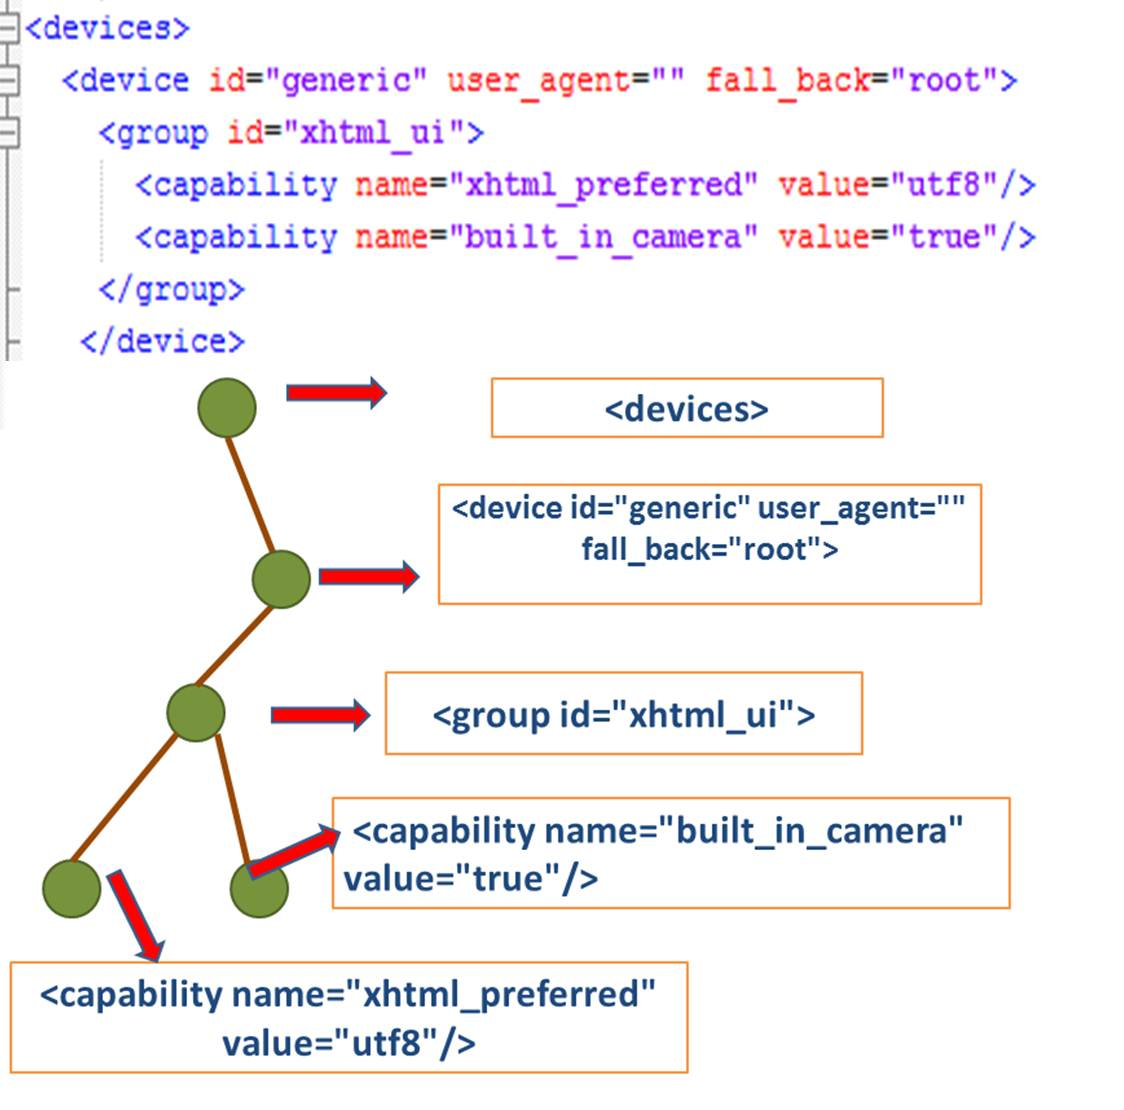
\includegraphics{imagenes/imagen1}
\end{center}
\caption {}
\label{Figura 1}
\end{figure}




\section{Opiniones acerca de Haskell}

Oswaldo Bayona: “Haskell me pareció un lenguaje muy bueno para el manejo de listas, debido a que tiene facilidades sintácticas como el ajuste de patrones y las guardas, que mejoran la capacidad de escritura y de lectura. Tiene muchas ventajas como que las funciones no presentan efectos secundarios ya que  no existen variables, además la recursión está optimizada, Haskell es perezoso;  en mi opinión no haber introducido el concepto de puntero u otra forma de referenciar presentó una dificultad considerable,  la forma en la que en Haskell se declaran nuevos  tipos de datos tampoco me parece tan buena;  pero la experiencia fue muy interesante y eso demuestra que  es bueno conocer varios lenguajes para resolver diversos problemas de formas mucho más eficientes y elegantes.”


\end{document}
